\documentclass[11pt,a4paper]{article}


\usepackage[toc,page]{appendix}
\usepackage{amsmath, amssymb}
\usepackage{bm}% bold math
\usepackage{cancel, caption}
\usepackage{dcolumn}% Align table columns on decimal point
\usepackage{epsfig, epsf}
\usepackage{graphicx,fancyhdr,natbib,subfigure}
\usepackage{lscape, longtable}
\usepackage{hyperref,ifthen}
\usepackage{verbatim}
\usepackage{color}
\usepackage[usenames,dvipsnames]{xcolor}
\usepackage{listings}
%% http://en.wikibooks.org/wiki/LaTeX/Colors



%%%%%%%%%%%%%%%%%%%%%%%%%%%%%%%%%%%%%%%%%%%
%       define Journal abbreviations      %
%%%%%%%%%%%%%%%%%%%%%%%%%%%%%%%%%%%%%%%%%%%
\def\nat{Nat} \def\apjl{ApJ~Lett.} \def\apj{ApJ}
\def\apjs{ApJS} \def\aj{AJ} \def\mnras{MNRAS}
\def\prd{Phys.~Rev.~D} \def\prl{Phys.~Rev.~Lett.}
\def\plb{Phys.~Lett.~B} \def\jhep{JHEP} \def\nar{NewAR}
\def\npbps{NUC.~Phys.~B~Proc.~Suppl.} \def\prep{Phys.~Rep.}
\def\pasp{PASP} \def\aap{Astron.~\&~Astrophys.} \def\araa{ARA\&A}
\def\jcap{\ref@jnl{J. Cosmology Astropart. Phys.}}%
\def\physrep{Phys.~Rep.}

\newcommand{\preep}[1]{{\tt #1} }

%%%%%%%%%%%%%%%%%%%%%%%%%%%%%%%%%%%%%%%%%%%%%%%%%%%%%
%              define symbols                       %
%%%%%%%%%%%%%%%%%%%%%%%%%%%%%%%%%%%%%%%%%%%%%%%%%%%%%
\def \Mpc {~{\rm Mpc} }
\def \Om {\Omega_0}
\def \Omb {\Omega_{\rm b}}
\def \Omcdm {\Omega_{\rm CDM}}
\def \Omlam {\Omega_{\Lambda}}
\def \Omm {\Omega_{\rm m}}
\def \ho {H_0}
\def \qo {q_0}
\def \lo {\lambda_0}
\def \kms {{\rm ~km~s}^{-1}}
\def \kmsmpc {{\rm ~km~s}^{-1}~{\rm Mpc}^{-1}}
\def \hmpc{~\;h^{-1}~{\rm Mpc}} 
\def \hkpc{\;h^{-1}{\rm kpc}} 
\def \hmpcb{h^{-1}{\rm Mpc}}
\def \dif {{\rm d}}
\def \mlim {m_{\rm l}}
\def \bj {b_{\rm J}}
\def \mb {M_{\rm b_{\rm J}}}
\def \mg {M_{\rm g}}
\def \qso {_{\rm QSO}}
\def \lrg {_{\rm LRG}}
\def \gal {_{\rm gal}}
\def \xibar {\bar{\xi}}
\def \xis{\xi(s)}
\def \xisp{\xi(\sigma, \pi)}
\def \Xisig{\Xi(\sigma)}
\def \xir{\xi(r)}
\def \max {_{\rm max}}
\def \gsim { \lower .75ex \hbox{$\sim$} \llap{\raise .27ex \hbox{$>$}} }
\def \lsim { \lower .75ex \hbox{$\sim$} \llap{\raise .27ex \hbox{$<$}} }
\def \deg {^{\circ}}
%\def \sqdeg {\rm deg^{-2}}
\def \deltac {\delta_{\rm c}}
\def \mmin {M_{\rm min}}
\def \mbh  {M_{\rm BH}}
\def \mdh  {M_{\rm DH}}
\def \msun {M_{\odot}}
\def \z {_{\rm z}}
\def \edd {_{\rm Edd}}
\def \lin {_{\rm lin}}
\def \nonlin {_{\rm non-lin}}
\def \wrms {\langle w_{\rm z}^2\rangle^{1/2}}
\def \dc {\delta_{\rm c}}
\def \wp {w_{p}(\sigma)}
\def \PwrSp {\mathcal{P}(k)}
\def \DelSq {$\Delta^{2}(k)$}
\def \WMAP {{\it WMAP \,}}
\def \cobe {{\it COBE }}
\def \COBE {{\it COBE \;}}
\def \HST  {{\it HST \,\,}}
\def \Spitzer  {{\it Spitzer \,}}
\def \ATLAS {VST-AA$\Omega$ {\it ATLAS} }
\def \BEST   {{\tt best} }
\def \TARGET {{\tt target} }
\def \TQSO   {{\tt TARGET\_QSO}}
\def \HIZ    {{\tt TARGET\_HIZ}}
\def \FIRST  {{\tt TARGET\_FIRST}}
\def \zc {z_{\rm c}}
\def \zcz {z_{\rm c,0}}

\newcommand{\ltsim}{\raisebox{-0.6ex}{$\,\stackrel
        {\raisebox{-.2ex}{$\textstyle <$}}{\sim}\,$}}
\newcommand{\gtsim}{\raisebox{-0.6ex}{$\,\stackrel
        {\raisebox{-.2ex}{$\textstyle >$}}{\sim}\,$}}
\newcommand{\simlt}{\raisebox{-0.6ex}{$\,\stackrel
        {\raisebox{-.2ex}{$\textstyle <$}}{\sim}\,$}}
\newcommand{\simgt}{\raisebox{-0.6ex}{$\,\stackrel
        {\raisebox{-.2ex}{$\textstyle >$}}{\sim}\,$}}

\newcommand{\Msun}{M_\odot}
\newcommand{\Lsun}{L_\odot}
\newcommand{\lsun}{L_\odot}
\newcommand{\Mdot}{\dot M}

\newcommand{\sqdeg}{deg$^{-2}$}
\newcommand{\lya}{Ly$\alpha$\ }
%\newcommand{\lya}{Ly\,$\alpha$\ }
\newcommand{\lyaf}{Ly\,$\alpha$\ forest}
%\newcommand{\eg}{e.g.~}
%\newcommand{\etal}{et~al.~}
\newcommand{\lyb}{Ly$\beta$\ }
\newcommand{\cii}{C\,{\sc ii}\ }
\newcommand{\ciii}{C\,{\sc iii}]\ }
\newcommand{\civ}{C\,{\sc iv}\ }
\newcommand{\SiIV}{Si\,{\sc iv}\ }
\newcommand{\mgii}{Mg\,{\sc ii}\ }
\newcommand{\feii}{Fe\,{\sc ii}\ }
\newcommand{\feiii}{Fe\,{\sc iii}\ }
\newcommand{\caii}{Ca\,{\sc ii}\ }
\newcommand{\halpha}{H\,$\alpha$\ }
\newcommand{\hbeta}{H\,$\beta$\ }
\newcommand{\hgamma}{H\,$\gamma$\ }
\newcommand{\hdelta}{H\,$\delta$\ }
\newcommand{\oi}{[O\,{\sc i}]\ }
\newcommand{\oii}{[O\,{\sc ii}]\ }
\newcommand{\oiii}{[O\,{\sc iii}]\ }
\newcommand{\heii}{[He\,{\sc ii}]\ }
\newcommand{\nv}{N\,{\sc v}\ }
\newcommand{\nev}{Ne\,{\sc v}\ }
\newcommand{\neiii}{[Ne\,{\sc iii}]\ }
\newcommand{\aliii}{Al\,{\sc iii}\ }
\newcommand{\siiii}{Si\,{\sc iii}]\ }


%%%%%%%%%%%%%%%%%%%%%%%%%%%%%%%%%%%%%%%%%%%%%%%%%%%%%
%              define Listings                       %
%%%%%%%%%%%%%%%%%%%%%%%%%%%%%%%%%%%%%%%%%%%%%%%%%%%%%
\definecolor{dkgreen}{rgb}{0,0.6,0}
\definecolor{gray}{rgb}{0.5,0.5,0.5}
\definecolor{mauve}{rgb}{0.58,0,0.82}

\lstset{frame=tb,
  language=Python,
  aboveskip=3mm,
  belowskip=3mm,
  showstringspaces=false,
  columns=flexible,
  basicstyle={\small\ttfamily},
  numbers=none,
  numberstyle=\tiny\color{gray},
  keywordstyle=\color{blue},
  commentstyle=\color{dkgreen},
  stringstyle=\color{mauve},
  breaklines=true,
  breakatwhitespace=true,
  tabsize=3
}

\begin{document}

\title{NPRs Python Notes}
\author{Nicholas P. Ross}
\date{\today}
\maketitle


%% Usually omit these for ApJ or MNRAS style files:


\begin{abstract}
The is my (NPR's) set of Python notes.  Things started as wanting to
just be an ``IDL to Python CheatSheet'', and have naturally and organically 
snowballed from there.  
%%
Suffice to say, when this document reached 47 pages long (and I started to 
take notes on how to do pytests ;-), this was no long a Cheat Sheet, and became 
something else; a general Python resource. \\

You will be able to find the latest version of these notes
and indeed the .tex file at:\\
\href{https://github.com/d80b2t/Research\_Notes}{\tt
https://github.com/d80b2t/Research\_Notes}.
\end{abstract}


\newpage
\tableofcontents
%\listoffigures
%\listoftables


\newpage
\section{The REAL Basics}

    \subsection{Versions}
    \$ python3
    \begin{lstlisting}
    Python 3.5.2 (v3.5.2:4def2a2901a5, Jun 26 2016, 10:47:25) 
    [GCC 4.2.1 (Apple Inc. build 5666) (dot 3)] on darwin
    Type "help", "copyright", "credits" or "license" for more information.
    >>> import numpy 
    >>> print (numpy.__version__)
    1.11.1 

    >>> import astropy 
    >>> print (astropy.__version__)
    1.2.1 
 
    >>> import sys
    >>> print (sys.version)
    3.5.2 (v3.5.2:4def2a2901a5, Jun 26 2016, 10:47:25) 
    [GCC 4.2.1 (Apple Inc. build 5666) (dot 3)]

    \end{lstlisting}
 

    \subsection{Style Guide for Python Code}
    \href{https://www.python.org/dev/peps/pep-0008/}{PEP 8 -- Style Guide for Python Code}.\\
    Use 4 spaces per indentation level.\\
    Python 3 disallows mixing the use of tabs and spaces for indentation.\\
    Code in the core Python distribution should always use \href{https://en.wikipedia.org/wiki/UTF-8}{UTF-8}. \\
    Imports should usually be on separate lines. \\
    Imports are always put at the top of the file, just after any module comments and docstrings, and before module globals and constants.\\
    Avoid extraneous whitespace in the following situations: Immediately inside parentheses, brackets or braces; Immediately before a comma, semicolon, or colon; Immediately before the open parenthesis that starts the argument list of a function call; {\it More than one space around an assignment (or other) operator to align it with another.}\\



    \subsection{Notebook}
    Click on the NBviewer...\\
    Then you can see the e.g. html of the notebook. \\
    But to change/execute it, then all you have to do is click the download button...\\
    Then put it on gitHub/Dropbox etc...\\
    (I need to learn about ``Tmox'' and ``SCreen'' Terminal emulators...)\\
  
    \noindent
    {\bf Run a code cell using Shift-Enter} or \\
    Alt-Enter runs the current cell and inserts a new one below.
    Ctrl-Enter run the current cell and enters command mode. 

    \noindent
    Google: ``ipython beyond plain python''\\
    
    http://nbviewer.ipython.org/github/fperez/cit2013/blob/master/06-IPython\%20-\%20beyond\%20plain\%20Python.ipynb

    iPython NB power = power of python + power of the command line with ``!'' + ``\%'' and ``\%\%'' ``magics''... 
    
http://nbviewer.ipython.org/github/ipython/ipython/blob/1.x/examples/notebooks/Part\%204\%20-\%20Markdown\%20Cells.ipynb

\begin{figure}
  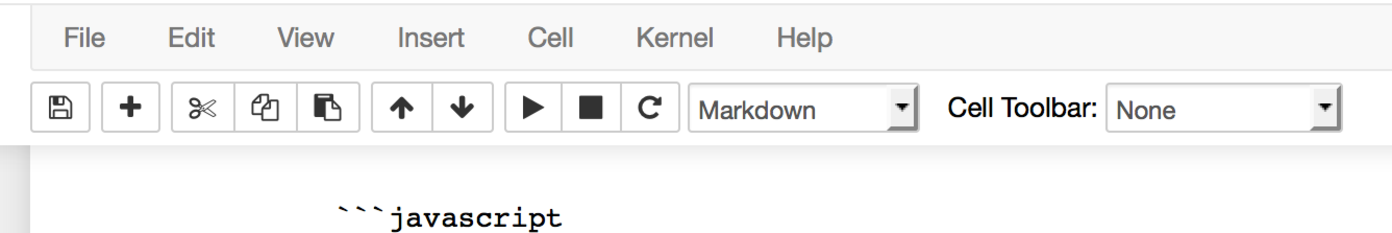
\includegraphics[height=4.0cm,width=14.0cm]
  {iPython_NB_toolbar.pdf}
  \centering
  \caption[]
  {Clicking on the Cell Toolbar ``Code'', ``Markdown'' etc. will power what happens in the Clells!!!}
  \label{fig:fig1}
\end{figure}
\href{https://github.com/profjsb/python-bootcamp}{https://github.com/profjsb/python-bootcamp}


\newpage
\section{The General Basics}
HEAVILY BORROWED/COPIED FROM: 
\href{http://shop.oreilly.com/product/0636920034919.do}{Python Data Science Handbook} by
\href{https://jakevdp.github.io/}{Jake VanderPlas}\footnote{Who is awesome, so stop being stingy and go buy his book!!! :-)}. 

\subsection*{Comments are marked by \#}

\subsection*{End-of-line Terminates a Statement}
\subsection*{Semicolon can Optionally Termnate a Statement}   

    \subsection*{Indentation: Whitespace Matters!}
    Indent code blocks by four spaces. 
    \begin{lstlisting}
      for i in range(100):
          # indentation indicates code block 
          total += i
    \end{lstlisting}
    
    \subsection*{Whitespace Within Lines Does Not Matter}

    \subsection*{Python Variables are Pointers}
    So when you write {\tt x=4}, you are essentially defining a {\it pointer} named {\tt x} which points to some memory bucket containing the value 4. Note one consequence of this: because Python variables just point to various objects, there is no need to ``declare'' the variable, or even require the variable to always point to information of the same type.  This is the sense in which people say Python is {\it dynamically-typed}: variable names can point to objects of any type.
    \begin{lstlisting}
      >>> x=[1,2,3]
      >>> y = x
      >>> print(y)
      [1, 2, 3]
      >>> x.append(4)    # add 4 to the end of x
      >>> print(y)           # y is modified as well!
      [1, 2, 3, 4]
      >>> x = 'something else'
      >>> print(y)         # y is unchanged. 
      [1, 2, 3, 4]
      >>> 
    \end{lstlisting}


    \subsection*{Everything is an Object}
    Python is an object-oriented programming language, and in Python
    everything is an object. Python is NOT a type-free language. Python
    has types; however, the types are linked not to the variable names but
    {\bf to the objects themselves}. When we say that everything in Python
    is an object, we really mean that everything is an object: even the
    attributes and methods of objects are themselves objects with their
    own type information:
    \begin{lstlisting}
      >>> x=4.0
      >>> x
      4.0
      >>> x.is_integer()
      True
      >>> type(x.is_integer)
      <class 'builtin_function_or_method'>
      >>> 
    \end{lstlisting}


    \subsection*{Operators}
    \subsubsection*{Identity Operators}
    \begin{lstlisting}
      >>> a = [1,2,3]
      >>> b = [1,2,3]
      >>> a == b
      True
      >>> a is b
      False
      >>> a is not b
      True
      >>> 
   \end{lstlisting}


    \subsection*{Conditional Statements: if-elif-else:}
        \begin{lstlisting}
          x=-15
          if  x==0:
              print(x, "is zero")
          elifx>0:
              print(x, "is positive")
          elifx<0:
              print(x, "is negative")
          else:
              print(x, "is unlike anything I've ever seen...")

          -15 is negative
      \end{lstlisting}


    \subsection*{for loops}
        \begin{lstlisting}
          >>> for i in range(10): 
          ...          print(i, end='  ')
          0 1 2 3 4 5 6 7 8 9 >>> 
          >>>
          >>>for i in range(10):
          ...        print(i, "\n")
          ... 
          0 
          
          1 
          
          2 
          .
          .
          .
          9 
        \end{lstlisting}


    \subsection*{}    




\newpage
\section{iPython}
\href{https://ipython.org/install.html}{https://ipython.org/install.html}\\

\smallskip
\smallskip
\noindent
{\tt \$ conda update ipython}\\

\smallskip
\smallskip
\noindent
{\tt \$ sudo pip3 install ipython[all] }\\
Then
{\tt \$ ipython3 notebook}\\

    \subsection{iPython from Fernando Perez}
    Try: tmpnb.org  {\bf VERY USEFUL}\\
    \href{http://www.pythonforbeginners.com/basics/ipython-a-short-introduction}{http://www.pythonforbeginners.com/basics/ipython-a-short-introduction}




\newpage
\section{Data Types}
{\tt int}, {\tt float}, {\tt complex}, {\tt bool}, {\tt str} and {\tt NoneType} are simple/scaler types. \\
{\tt list}, {\tt tuple}, {\tt dict} and {\tt set} are Data Structures. \\

%% \subsection{e.g. Data types}
\begin{lstlisting}
>>> n = 123               # int, integers
>>> f = 123.               # floats,  floating-point: i.e. real numbers
>>> L = [1,2,3]           
>>> a = (1,2,3)
>>> D = {1,2,3}
>>> x = {'1': '2', '3': 45}
>>> s = '1,2,3'

>>> b = True               # boolean: True/False values
>>> nt = None            # special object indicating nulls

>>> type(n)
<class 'int'>
>>> type(f)
<class 'float'>
>>> type(L)
<class 'list'>
>>> type(a)
<class 'tuple'>
>>> type(D)
<class 'set'>
>>> type(x)
<class 'dict'>
>>> type(s)
<class 'str'>

>>> type(b)
<class 'bool'>
>>> type(nt)
<class 'NoneType'>
\end{lstlisting}


    \subsection{Lists}

    \subsection{tuple}
    
    \subsection{Dictionaries}
    \begin{lstlisting}
      >>> x = {'hello': 'Zed', 'name': 45}
      >>> x['hello']
      'Zed'
      >>> 
    \end{lstlisting}
    
    \subsection{set}

    \subsection{Pandas and {\tt DataFrames}}
    \begin{lstlisting}
      import numpy
      import matplotlib.pyplot as plt
      import re
      import pandas as pd 
      
      # The data directory PATH
      data_dir = "/cos_pc19a_npr/data/WISE/W4/"
      
      # The data directory FILENAME
      data_file="WISE_W4_W4SNRge3_W4MPROlt4.0_nohdr.tbl"
      
      data_in = data_dir+data_file
      
      cols = ['designation', 'ra', 'dec', 'sigra', 'sigdec', 'w1mpro', 'w1sigmpro', 'w1snr', 'w2mpro', 'w2sigmpro', 'w2snr', 'w3mpro', 'w3sigmpro', 'w3snr', 'w4mpro', 'w4sigmpro', 'w4snr', 'w4rchi2']
      
      df = pd.read_table(data_in) 
      
      ##
      print(list(df.columns.values))
      
      ## 
      print(type(df))
    \end{lstlisting}
    
    \begin{lstlisting}
      In [5]: type(df)
      Out[5]: pandas.core.frame.DataFrame
    \end{lstlisting}

    


\newpage
\section{String Manipulation and Regular Expressions}






\newpage
\section{A general code example ;-)} 

\begin{lstlisting}
"""
Outline:

You have a certain amount of credit to spend at a book store. You want to buy two books and you want to spend all of your store credit. However, you have to carry the books a far distance so you want to buy the lightest pair of books possible.
Each book available in the bookstore is represented as a tuple of their price and weight. You are given a list of all books in the bookstore as follows:
[(price0, weight0), (price1, weight1), etc, (priceN, weightN)]
Print the indices of the two books you should buy and their combined weight.
"""
    
    
credit = 18
books = [(17, 5), (3, 55), (5, 12), (14, 9), (16, 1), (9, 5),
         (5, 6), (18, 13), (19, 7), (1, 20), (4, 12), (11, 1),
         (8, 6), (8, 18), (3, 4), (13, 7), (17, 22), (20, 7)]


# Point 1: Strong condition: PriceBookA + PriceBookB = 18. 

# Want to take the LIST of books, it's not a long list, so happy to loop over -- indeed happy to loop over twice if needs be. 

# Then generate a new list, goodPrice, of the pairs of books that have PriceBookA + PriceBookB = 18
goodPrice=[]
largeWeight = 100000.

for i in range(len(books)):
    PriceBookA =  books[i][0] 
    for j in range(len(books)):
        PriceBookB =  books[j][0] 
        
        if ((PriceBookA + PriceBookB) == 18) and (i != j):
            # goodPrice becomes the sum of the weights 
            # if the sum of the weights of the books is less than largeWeight then (i) keep that sum and (ii) keep the indicies and then (iiI) set largeWeight to the new min weight. 
            
            sumWeights = books[i][1]+books[j][1]
            if (sumWeights < largeWeight):
                largeWeight = sumWeights
                goodIndexA = i     
                goodIndexB = j            
        
#            goodPrice.append(books[i][1]+ )
print(largeWeight) 
print(goodIndexA)
print(goodIndexB)


# Figure out which (limited) combinations of books satifisy this price condition

# Sort that set by sum of weights (WeightBookA + WeightBookB). Pick the minimum there. 

\end{lstlisting}


    


\newpage
\section{Britton's Classes :-)}

\subsection{``If lost in the desert...''}
$>>>$ dir(thing) \\
$>>>$ dir(thing) \\

%% http://tex.stackexchange.com/questions/45981/square-brackets-in-math-mode-without-the-bracket-symbols

%%   Symbols in Python    % + - = ! / ( ) [ ] < > | ' :


\subsection{Lists}
\begin{lstlisting}
>>> super_list = [0, [3,4,5], "Hello World!", range(5)] 
>>> print super_list 

[0, [3, 4, 5], 'Hello World!', [0, 1, 2, 3, 4]] 
>>> print super_list[1] 
[3, 4, 5] 
>>> print super_list[-1]
[0, 1, 2, 3, 4] 
>>> print super_list[1[0]] 
Traceback (most recent call last):
  File "<stdin>", line 1, in <module>
TypeError: 'int' object is not subscriptable
>>> print super_list[1][0] 
  3

>>> c = range(10) 
>>> print c 
[0, 1, 2, 3, 4, 5, 6, 7, 8, 9]
>>> c.append(range(3)) 
>>> print c 
[0, 1, 2, 3, 4, 5, 6, 7, 8, 9, [0, 1, 2]]
>>> c.extend(range(3)) 
>>> print c 
[0, 1, 2, 3, 4, 5, 6, 7, 8, 9, [0, 1, 2], 0, 1, 2]
>>> del c[4]
>>> print c
[0, 1, 2, 3, 5, 6, 7, 8, 9, [0, 1, 2], 0, 1, 2]

>>> z =  [42]*5
>>> [42, 42, 42, 42, 42]

>>> print super_list
[0, [3, 4, 5], 'Hello World!', [0, 1, 2, 3, 4]]
>>> print len(super_list)
4
>>> print len(super_list[-1])
5
\end{lstlisting}


\subsection{Dictionaries and Maps}
From: \href{http://learnpythonthehardway.org/book/ex39.html}{http://learnpythonthehardway.org/book/ex39.html}: 
You are now going to learn about the Dictionary data structure in
Python. A Dictionary (or "dict") is a way to store data just like a
list, but instead of using only numbers to get the data, you can use
almost anything. This lets you treat a dict like it's a database for
storing and organizing data.

From: \href{https://docs.python.org/3/tutorial/datastructures.html\#dictionaries}{https://docs.python.org/3/tutorial/datastructures.html\#dictionaries}: 
Another useful data type built into Python is the dictionary (see
Mapping Types — dict). Dictionaries are sometimes found in other
languages as “associative memories” or “associative arrays”. Unlike
sequences, which are indexed by a range of numbers, dictionaries are
indexed by keys, which can be any immutable type; strings and numbers
can always be keys. Tuples can be used as keys if they contain only
strings, numbers, or tuples; if a tuple contains any mutable object
either directly or indirectly, it cannot be used as a key. You can’t
use lists as keys, since lists can be modified in place using index
assignments, slice assignments, or methods like append() and extend().

It is best to think of a dictionary as an unordered set of key: value
pairs, with the requirement that the keys are unique (within one
dictionary). A pair of braces creates an empty dictionary: {}. Placing
a comma-separated list of key:value pairs within the braces adds
initial key:value pairs to the dictionary; this is also the way
dictionaries are written on output.

The main operations on a dictionary are storing a value with some key
and extracting the value given the key. It is also possible to delete
a key:value pair with del. If you store using a key that is already in
use, the old value associated with that key is forgotten. It is an
error to extract a value using a non-existent key.

\begin{lstlisting}
# http://www.tutorialspoint.com/python/python_dictionary.htm
dict = {'Name': 'Zara', 'Age': 7, 'Class': 'First'}
print("dict['Name']: ", dict['Name'])
print("dict['Age']: ", dict['Age'])
print("dict['Alice']: ", dict['Alice]')
\end{lstlisting}

\noindent
From: \href{http://openbookproject.net/thinkcs/python/english3e/dictionaries.html}{http://openbookproject.net/thinkcs/python/english3e/dictionaries.html}:

Hashing. The order of the pairs may not be what was expected. Python uses complex algorithms, designed for very fast access, to determine where the key:value pairs are stored in a dictionary. For our purposes we can think of this ordering as unpredictable.
You also might wonder why we use dictionaries at all when the same concept of mapping a key to a value could be implemented using a list of tuples:
\begin{lstlisting}
>>> {"apples": 430, "bananas": 312, "oranges": 525, "pears": 217}
{'pears': 217, 'apples': 430, 'oranges': 525, 'bananas': 312}
>>> [('apples', 430), ('bananas', 312), ('oranges', 525), ('pears', 217)]
[('apples', 430), ('bananas', 312), ('oranges', 525), ('pears', 217)]
\end{lstlisting}

The reason is dictionaries are very fast, implemented using a
technique called hashing, which allows us to access a value very
quickly. By contrast, the list of tuples implementation is slow. If we
wanted to find a value associated with a key, we would have to iterate
over every tuple, checking the 0th element. What if the key wasn’t
even in the list? We would have to get to the end of it to find out.


\newpage
\section{Packages}

\subsection{Install packages}

\noindent
To install: \\
{\tt python3 -m pip install somepackage}


\subsection{Key Packages}
{\tt
astropy \\
% astroscrappy \\
healpy\\
ipython \\ 
matplotib\\
nose \\
numpy\\
pandas \\
reproject\\
scipy \\
sympy \\ 
%pyds9\\
pyFITS\\
yt\\
}


\subsection{PyPI - the Python Package Index}
\noindent
\href{https://pypi.python.org/pypi}{https://pypi.python.org/pypi}

\noindent
The Python Package Index is a repository of software for the Python
programming language. There are currently 85904 packages
here\footnote{As of Fri Aug 5 13:37:24 PDT 2016.}.



\newpage
\section{Class vs. an Instance}
Difference between a class and an instance is an Object Oriented (OO)
concept.

Python and Ruby both recommend {\tt UpperCamelCase} for class names,
{\tt CAPITALIZED\_WITH\_UNDERSCORES} for constants, and {\tt
lowercase\_separated\_by\_underscores} for other names.  
%% see also https://en.wikipedia.org/wiki/Naming_convention\_(programming)

And {\tt snake\_case} for variable names, function names, and method names. 

Generally speaking, instance variables are for data unique to each instance and class variables are for attributes and methods shared by all instances of the class:

Definitions: 
from \href{http://www.tutorialspoint.com/python/python\_classes\_objects.htm}{http://www.tutorialspoint.com/python/python\_classes\_objects.htm}
\begin{itemize}
\item{Class: A user-defined prototype for an object that defines a set of
    attributes that characterize any object of the class. The attributes
    are data members (class variables and instance variables) and methods,
    accessed via dot notation.}

  %A blueprint defining the charactaristics and behaviors of an object of that class type. Class names should be written in CamelCase, starting with a capital letter.

\item{Instance variable: A variable that is defined inside a method
    and belongs only to the current instance of a class.}

\item{Inheritance: The transfer of the characteristics of a class to
    other classes that are derived from it.}
\end{itemize}

Maybe see also \href{http://stackoverflow.com/questions/114214/class-method-differences-in-python-bound-unbound-and-static}{http://stackoverflow.com/questions/114214/class-method-differences-in-python-bound-unbound-and-static}. 


    \subsection{Abstract Classes}
    \href{https://www.hackerrank.com/challenges/30-abstract-classes/tutorial}{https://www.hackerrank.com/challenges/30-abstract-classes/tutorial} \\

    \textbf{\textsc{Case Study: Abstraction:}}
    This is is an essential feature of object-oriented programming. In essense, it's the separation between what a class does and how it's accomplished. 

One real world example of this concept is a snack machine, where you
give the machine money, make a selection, and the machine dispenses
the snack. The only thing that matters is what the machine does (i.e.:
dispenses the selected snack); you can easily buy a snack from any
number of snack machines without knowing how the machine's internals
are designed (i.e.: the implementation details).

Abstract Class This type of class can have abstract methods as well as
defined methods, but it cannot be instantiated (meaning you cannot
create a new instance of it). To use an abstract class, you must
create and instantiate a subclass that extends the abstract class. Any
abstract methods declared in an abstract class must be implemented by
its subclasses (unless the subclass is also abstract).

 abc -- Abstract Base Classes
Source code: Lib/abc.py

This module provides the infrastructure for defining abstract base classes (ABCs) in Python, as outlined in PEP 3119; see the PEP for why this was added to Python. (See also PEP 3141 and the numbers module regarding a type hierarchy for numbers based on ABCs.)

The collections module has some concrete classes that derive from ABCs; these can, of course, be further derived. In addition the collections.abc submodule has some ABCs that can be used to test whether a class or instance provides a particular interface, for example, is it hashable or a mapping.




\newpage
\section{Functions}
{\bf N.B.} Straight from: \href{http://www.python-course.eu/python3\_functions.php}{http://www.python-course.eu/python3\_functions.php}. 

The concept of a function is one of the most important ones in
mathematics. A common usage of functions in computer languages is to
implement mathematical functions. Such a function is computing one or
more results, which are entirely determined by the parameters passed
to it.

In the most general sense, a function is a structuring element in
programming languages to group a set of statements so they can be
utilized more than once in a program. The only way to accomplish this
without functions would be to reuse code by copying it and adapt it to
its different context. Using functions usually enhances the
comprehensibility and quality of the program. It also lowers the cost
for development and maintenance of the software.

Functions are known under various names in programming languages,
e.g. as subroutines, routines, procedures, methods, or subprograms.

A function in Python is defined by a def statement. The general syntax looks like this:
\begin{lstlisting}
def function-name(Parameter list):
    statements, i.e. the function body
\end{lstlisting}

The parameter list consists of none or more parameters. Parameters are
called arguments, if the function is called. The function body
consists of indented statements. The function body gets executed every
time the function is called.

Parameter can be mandatory or optional. The optional parameters (zero
or more) must follow the mandatory parameters.

Function bodies can contain one or more return statement. They can be
situated anywhere in the function body. A return statement ends the
execution of the function call and "returns" the result, i.e. the
value of the expression following the return keyword, to the
caller. If the return statement is without an expression, the special
value None is returned. If there is no return statement in the
function code, the function ends, when the control flow reaches the
end of the function body and the value value will be returned.
Example:

\begin{lstlisting}
def fahrenheit(T_in_celsius):
    """ returns the temperature in degrees Fahrenheit """
    return (T_in_celsius * 9 / 5) + 32

for t in (22.6, 25.8, 27.3, 29.8):
    print(t, ": ", fahrenheit(t))
\end{lstlisting}

The output of this script looks like this:
\begin{lstlisting}
22.6 :  72.68
25.8 :  78.44
27.3 :  81.14
29.8 :  85.64
\end{lstlisting}

\noindent
Optional Parameters.\\
Functions can have optional parameters, also called default
parameters. Default parameters are parameters, which don't have to be
given, if the function is called. In this case, the default values are
used. We will demonstrate the operating principle of default
parameters with an example. The following little script, which isn't
very useful, greets a person. If no name is given, it will greet
everybody:

\begin{lstlisting}
def Hello(name="everybody"):
    """ Greets a person """
    print("Hello " + name + "!")

Hello("Peter")
Hello()
\end{lstlisting}

\noindent
The output looks like this:

\begin{lstlisting}
Hello Peter!
Hello everybody!
\end{lstlisting}

\noindent
Docstring.\\
The first statement in the body of a function is usually a string, which can be accessed with {\tt function\_name.\_\_doc\_\_}. This statement is called Docstring. Example:

\begin{lstlisting}
def Hello(name="everybody"):
    """ Greets a person """
    print("Hello " + name + "!")

print("The docstring of the function Hello: " + Hello.__doc__)
\end{lstlisting}

\noindent 
The output:
\begin{lstlisting}
The docstring of the function Hello:  Greets a person 
\end{lstlisting}






\newpage
\section{Errors and fixes}
    \subsection{NameError}
    Error message: ``NameError: name 'now' is not defined''\\
    Solution: Use raw\_input() for python2 and input() in python3. In python2, input() is the same as saying eval(raw\_input()) \\ 
%% http://stackoverflow.com/questions/15190632/nameerror-name-now-is-not-defined







\newpage
\section{IDL to Python}
Key links:\\
\href{http://www.johnny-lin.com/cdat_tips/tips_array/idl2num.html}{IDL to Numeric/numarray Mapping}\\
\href{http://www.astro.umd.edu/~mbk/idl-numpy.html}{NumPy for IDL users}\\

\href{http://mathesaurus.sourceforge.net/idl-numpy.html}{http://mathesaurus.sourceforge.net/idl-numpy.html}\\

\href{http://mathesaurus.sourceforge.net/idl-python-xref.pdf}{http://mathesaurus.sourceforge.net/idl-python-xref.pdf}\\

\begin{table}
  \begin{center}
    \setlength{\tabcolsep}{4pt}
    \begin{tabular}{ll}
      \hline\hline
      IDL code   & Python code \\
      \hline 
      .run 'foo.pro'  & exec(open("./findSecondLargestNo.py").read())\\
                            & \%run my\_script.py  ({\tt ipython} only??)\\
      \hline
      data=READFITS('file',header) 	 & data=pyfits.open('file')\\
      tdata  = mrdfits('SpIESch1ch2.fits',0, hdr) 	 & tdata = data[0].data \\
      tbdata = mrdfits('SpIESch1ch2.fits',1, hdr) 	 & tdata = data[1].data \\
      help, tbdata, /str     & info(tbdata)\\
      print, size(tbdata)  & shape(tbdata)\\
      print, tbdata[0].flux\_aper\_1 & print tbdata.FLUX\_APER\_1[0]\\
      help, tbdata.flux\_aper\_1        & tbdata.FLUX\_APER\_1? \\
      fluxaper = tbdata.flux\_aper\_1[2] & fluxaper = ??? \\
      \hline 
     {\it (using fitsio)} & d = fitsio.read('SpIESch1ch2.fits',1) \\
      \hline
      \label{tab:IDL2Python}
    \end{tabular}
    \caption{IDL to Python}
    \label{table:idl_vs_python}
  \end{center}
\end{table}



%%%%%%%%%%%%%%%%%%%%%%%%%%%%%%%%%%%%%%%%%%%
%%%%%%%%%%%%%%%%%%%%%%%%%%%%%%%%%%%%%%%%%%%
%%
%%      I N P U T
%%
%%%%%%%%%%%%%%%%%%%%%%%%%%%%%%%%%%%%%%%%%%%
%%%%%%%%%%%%%%%%%%%%%%%%%%%%%%%%%%%%%%%%%%%
\newpage
\section{INPUT}
Just some general ways to get variables read-in and different 'tricks' to Python3 input. \\
\href{https://en.wikibooks.org/wiki/Non-Programmer\%27s\_Tutorial\_for\_Python\_3/File\_IO}{https://en.wikibooks.org/wiki/Non-Programmer\%27s\_Tutorial\_for\_Python\_3/File\_IO}\\
\href{http://www.programiz.com/python-programming/file-operation}{http://www.programiz.com/python-programming/file-operation}\\
\href{http://stackoverflow.com/questions/3925614/how-do-you-read-a-file-into-a-list-in-python}{http://stackoverflow.com/questions/3925614/how-do-you-read-a-file-into-a-list-in-python}\\


\begin{lstlisting}
>>> s = eval(input())
>>> s = input().split()
asdf asdfasdf ddddf aa
>>> s
['asdf', 'asdfasdf', 'ddddf', 'aa']
\end{lstlisting}

\begin{lstlisting}
>>> x, y, z, n = int(eval(input())), int(eval(input())), int(eval(input())), int(eval(input()))
>>> x, y, z, n = (int(eval(input())) for _ in range(4))
\end{lstlisting}

Would like some code to read in .dat files...
\begin{lstlisting}
# Would like some code to read in .dat files...
with open('million_nos.dat') as f:
    lines = f.read().splitlines()
\end{lstlisting}

\begin{lstlisting}
data = [line.strip() for line in open("million_nos.dat", 'r')]
## Still need to test this...
\end{lstlisting}

%% # Would like some code to read in .csv files...
%% # Would like some code to read in .txt files...

\smallskip
\smallskip
\noindent 
Would like some code to read in .FITS files... -- see~\ref{sec:FITS}. 
\begin{lstlisting}
\end{lstlisting}


    \subsection{e.g. running a script from the Command Line}
    \begin{lstlisting}
   from sys import argv
   # I want the "argument vector" from the system module

   # When running script, you now expect/need three (additional) inputs/arguments..
   script, first, second, third = argv

   print("The script is called:", script)
   print("Your first variable is:", first)
   print("Your second variable is:", second)
   print("Your third variable is:", third)
   \end{lstlisting}



\newpage
\section{FITS Files}\label{sec:FITS}


\begin{lstlisting}
#!/usr/bin/python

"""
Some baby code just to start to play around with FITS files in Python and AstroPy and
make some QSO color-color plots... ;-)
"""

"""
Links to FITS resources:
  http://docs.astropy.org/en/stable/io/fits/
  http://www.astropy.org/astropy-tutorials/FITS-images.html
  https://python4astronomers.github.io/astropy/fits.html
  https://gist.github.com/phn/3054997
  http://www.astropython.org/tutorials/pyfits-fits-files-in-python93/
"""

import numpy
import matplotlib.pyplot as plt
import pyfits

# Set the path to, and the name of, your data FITS file 
data_path='/cos_pc19a_npr/data/DECaLS/'
data_file='decals-dr2-DR12Q.fits'

# 'data_full' just a variable name that NPR likes to use ;-)
data_full=data_path+data_file

# Reading in and seeing  the Header information
pyfits.info(data_full)

header_primary = pyfits.getheader(data_full)
list(header_primary.keys())

# Open, and get info on, the FITS file:
hdulist = pyfits.open(data_full)
hdulist.info()

# Okay, what we really want to do... ;-) 
data_table = pyfits.getdata(data_full)

# Quick check on the format/dimensions of the FITS table file...
print(type(data_table),'\n')
print('The number of rows of is.... ', data_table.shape,'\n')
print('The number of columns is...  ', len(data_table.names),'\n\n')

## Interograting the FITS file...
# First row
print(data_table[0])

# First column
print(data_table.field(0))

# First row, First column
print(data_table[0][0])

# Names of individual columns
print(data_table.names, '\n\n')

##
## Now getting into it some more...
##

decam_flux = data_table.field('DECAM_FLUX')

print(numpy.ndarray.max(decam_flux))

numpy.histogram(decam_flux)

plt.hist(decam_flux, bins='auto')
plt.show()
\end{lstlisting}




%%%%%%%%%%%%%%%%%%%%%%%%%%%%%%%%%%%%%%%%%%%
%%%%%%%%%%%%%%%%%%%%%%%%%%%%%%%%%%%%%%%%%%%
%%
%%      O U T P U T
%%
%%%%%%%%%%%%%%%%%%%%%%%%%%%%%%%%%%%%%%%%%%%
%%%%%%%%%%%%%%%%%%%%%%%%%%%%%%%%%%%%%%%%%%%
\newpage
\section{OUTPUT}
For the ``write'' statement, I think you have to put everything into 
a string format, otherwise it just barfs... \\
\href{http://learnpythonthehardway.org/book/ex16.html}{http://learnpythonthehardway.org/book/ex16.html}

\noindent
\begin{lstlisting}
import random

size = 1000000
lis = random.sample(range(size), size)

outfile = open('temp.dat', 'w')
for i in range(len(lis)):
    outfile.write(str(lis[i])+'\n')
    
outfile.close()
\end{lstlisting}

\begin{lstlisting}
  outfile = open('WISE_spectra_triples_4wget_temp.dat', 'w') \\
  for i in range(len(ra)): 
    print i, ra[i] 
    plate_out = str(plate[i])
    mjd_out = str(mjd[i]) 
    fiberid_out = str(fiberid[i])

    outfile.write(plate_out+"/spec-"+plate_out+"-"+mjd_out+"-"+fiberid_out.zfill(4)+".fits \n")
\end{lstlisting}





\newpage
\section{IDL Where}
As always (!! ;-) there are many different ways to do something in
Python3 for the equivalent in IDL. The IDL Where command is no
exception...

    \subsection{{\tt a in b}}.


    \subsection{numpy where}
      Generating Indices: np.where
    \begin{lstlisting}
      import numpy as np
      rand = np.random.RandomState(42)
      X = rand.randint(10, size=(3, 4))
      X[np.where(X % 2 == 0)]
    \end{lstlisting}


\newpage
\section{v2 vs. v3}
\href{https://docs.python.org/3.0/library/2to3.html}{https://docs.python.org/3.0/library/2to3.html}\\
\href{https://docs.python.org/3/howto/pyporting.html}{https://docs.python.org/3/howto/pyporting.html}\\
\href{https://docs.python.org/3/howto/pyporting.html}{https://docs.python.org/3/howto/pyporting.html}
\href{https://docs.python.org/2/library/2to3.html}{https://docs.python.org/2/library/2to3.html}\\
\$ {\tt 2to3 -w example.py}\\


    \subsection{print}
    {\tt print a} vs. {\tt print (a)}
    Thus, just use () all the time!!
    
    \subsection{Division}
    / = truncating (integer floor) division in P2.x when using ints; float division in P3.x
    // = truncating div in P2.x, P3.x 
    

     \subsection{Unbound Methods}
     As of Python 3.0: The concept of ``unbound methods'' has been
removed from the language. When referencing a method as a class
attribute, you now get a plain function object. So this example is
valid python 3.X code, since there are no ``unbound methods'', just
functions attached to class objects.  %% - Dagoth Ulen Sep 26 '13 at
20:09

     {\tt \$ python}
    \begin{lstlisting}
   Python 2.7.11 |Anaconda 2.5.0 (x86_64)| (default, Dec  6 2015, 18:57:58) 
   [GCC 4.2.1 (Apple Inc. build 5577)] on darwin
   Type "help", "copyright", "credits" or "license" for more information.
   >>> import mystuff
   >>> mystuff.tangerine
    'Living reflection of a dream'
   >>> mystuff.MyStuff
    <class 'mystuff.MyStuff'>
   >>> mystuff.MyStuff.apple
    <unbound method MyStuff.apple>
     \end{lstlisting}

     {\tt \$ python3}
    \begin{lstlisting}
   Python 3.5.2 (v3.5.2:4def2a2901a5, Jun 26 2016, 10:47:25) 
   [GCC 4.2.1 (Apple Inc. build 5666) (dot 3)] on darwin
   Type "help", "copyright", "credits" or "license" for more information.
   >>> import mystuff
   >>> mystuff.tangerine
    'Living reflection of a dream'
   >>> mystuff.MyStuff
    <class 'mystuff.MyStuff'>
   >>> mystuff.MyStuff.apple
    <function MyStuff.apple at 0x1013499d8>
    \end{lstlisting}




\newpage
\section{Linear Algebra}
\href{http://docs.scipy.org/doc/scipy/reference/tutorial/linalg.html}{http://docs.scipy.org/doc/scipy/reference/tutorial/linalg.html}

\begin{lstlisting}
import numpy as np
from scipy import linalg
A = np.array([[1,2],[3,4]])
linalg.inv(A)
A.dot(linalg.inv(A)) #double check
\end{lstlisting}

\noindent
\href{https://twitter.com/SciPyTip/status/756510468160774144}{https://twitter.com/SciPyTip/status/756510468160774144}
You can solve a linear system {\bf Ax = b} with {\tt linalg.solve(A, b)}.
\begin{lstlisting}

\end{lstlisting}





\newpage
\section{Pytests}
\subsection{High-level Overview}
pytest: helps you write better programs
The pytest framework makes it easy to write small tests, yet scales to support complex functional testing for applications and libraries.

``pytest is a mature full-featured Python testing tool that helps you write better programs.''

\href{http://docs.pytest.org/en/latest/}{http://docs.pytest.org/en/latest/}

Getting started: \href{http://docs.pytest.org/en/latest/getting-started.html}{http://docs.pytest.org/en/latest/getting-started.html}

\href{pytest Documentation (Release 3.0.2.dev)}{https://media.readthedocs.org/pdf/pytest/latest/pytest.pdf}

\href{http://docs.pytest.org/en/latest/contents.html}{http://docs.pytest.org/en/latest/contents.html}

\subsection{Example of a (very) simple test:}

An example of a simple test:
\begin{lstlisting}
# content of test_sample.py
def func(x):
    return x + 1

def test_answer():
    assert func(3) == 5
To execute it:
\end{lstlisting}


\begin{figure}
  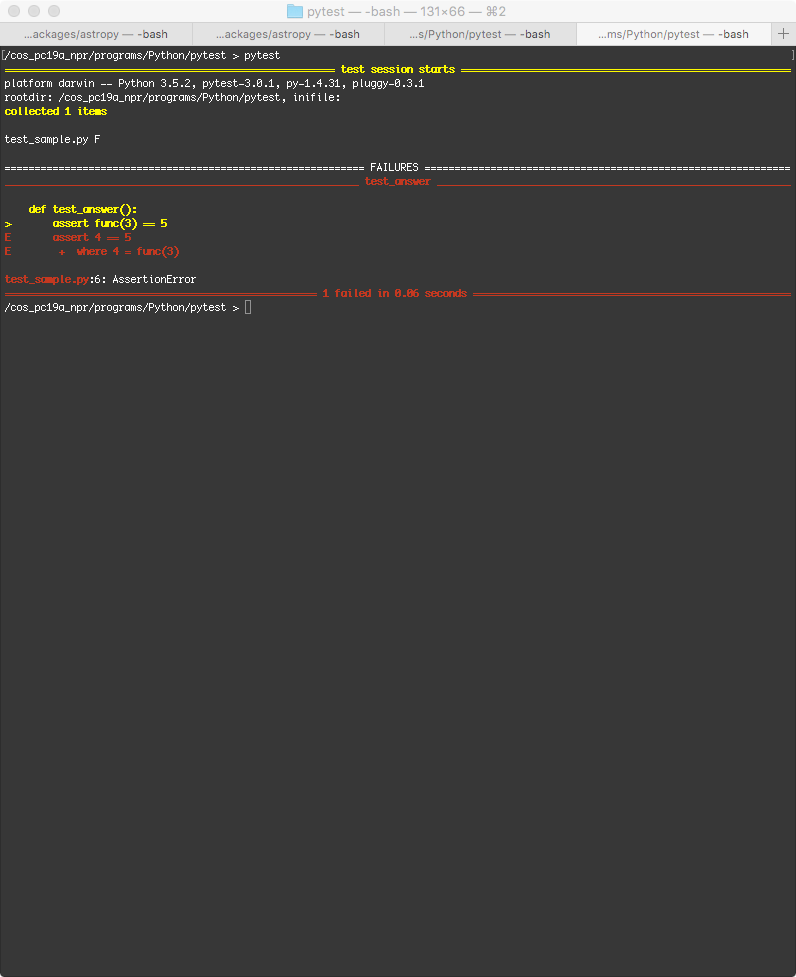
\includegraphics [height=14.0cm,width=10.0cm]
  {pytest_screengrab.png}
  \centering
  \caption[]{}
  \label{fig:fig2}
\end{figure}


\noindent
{\tt \$ pytest}
\begin{lstlisting}
======= test session starts ========
collected 1 items

test_sample.py F

======= FAILURES ========
_______ test_answer ________

    def test_answer():
>       assert func(3) == 5
E       assert 4 == 5
E        +  where 4 = func(3)

test_sample.py:5: AssertionError
======= 1 failed in 0.12 seconds ========
\end{lstlisting}

Due to pytest‘s detailed assertion introspection, only plain assert
statements are used. See Getting Started for more examples.





\newpage
\section{Plots}

From \href{http://stackoverflow.com/questions/16522380/python-pandas-plot-is-a-no-show}{http://stackoverflow.com/questions/16522380/python-pandas-plot-is-a-no-show}: 
Put
\begin{lstlisting}
import matplotlib.pyplot as plt
\end{lstlisting}
at the top, and
\begin{lstlisting}
plt.show()
\end{lstlisting}
at the end.



\newpage
\section{Pandas}
{\bf (So.... this might well get split off into its separate
document...)}


\smallskip
\smallskip
\noindent 
\begin{lstlisting}
import numpy
import matplotlib.pyplot as plt
import re
import pandas as pd 

# The data directory PATH
data_dir = "/cos_pc19a_npr/data/WISE/W4/"

# The data directory FILENAME
data_file="WISE_W4_W4SNRge3_W4MPROlt4.0_nohdr.tbl"

data_in = data_dir+data_file

cols = ['designation', 'ra', 'dec', 'sigra', 'sigdec', 'w1mpro', 'w1sigmpro', 'w1snr', 'w2mpro', 'w2sigmpro', 'w2snr', 'w3mpro', 'w3sigmpro', 'w3snr', 'w4mpro', 'w4sigmpro', 'w4snr', 'w4rchi2']

## If using a file *WITH* a header
# df = pd.read_table(data_in, header=54) 

df = pd.read_table(data_in) 
\end{lstlisting}

\smallskip
\smallskip
\noindent 
So, pandas tends to work in these things called {\tt DataFrames}. 
I (currently) don't understand DataFrames :-/




































































\newpage
\section{Gotchas}
``follow up: PYTHONPATH is a hazardous environment variable, and should never include one Python's site-packages'' 
%% <blockquote class="twitter-tweet" lang="en"><p><a href="https://twitter.com/npr247">@npr247</a> <a href="https://twitter.com/jakevdp">@jakevdp</a> <a href="https://twitter.com/demitrimuna">@demitrimuna</a> follow up: PYTHONPATH is a hazardous environment variable, and should never include one Python\&#39;s site-packages</p>\&mdash; Min RK (@minrk) <a href="https://twitter.com/minrk/status/555137558850453505">January 13, 2015</a></blockquote><script async src="//platform.twitter.com/widgets.js" charset="utf-8"></script>

See 429 in history\_20150113.txt and onwards... :-) 

%> echo \$PYTHONPATH 
%:/Users/npr1/boss/products/Darwin/sdss3tools/v1_7_4/python:/cos_pc19a_npr/BOSS/esutil/esutil/lib/python2.7/site-packages/:/cos_pc19a_npr/BOSS/pydl/:/Users/npr1/boss/products/eups/bin



\newpage
\section{A few General Notes}
    \subsection{What's the difference between raw\_input() and input()?}
    The difference is that {\tt raw\_input()} does not exist in Python 3.x,
    while {\tt input()} does. Actually, the old {\tt raw\_input()} has been renamed to
     {\tt input()}, and the old  {\tt input()} is gone (but can easily be simulated by
    using  {\tt eval(input())}).
    Reference: \href{http://stackoverflow.com/questions/4915361/whats-the-difference-between-raw-input-and-input-in-python3-x}{http://stackoverflow.com/questions/4915361/whats-the-difference-between-raw-input-and-input-in-python3-x}. 
   

    \subsection{Loops}
    \begin{lstlisting}
   n = eval(input())
   for _ in range(n):
      <indented code here>
  \end{lstlisting}


    \subsection{List Comprehensions}
    \begin{lstlisting}
   >>> ListOfNumbers = [ x for x in range(10) ] # List of integers from 0 to 9
   >>> ListOfNumbers

   >>> ListOfThreeMultiples = [x for x in range(100) if x % 3 == 0] # Multiples of 3 below 10
   >>> ListOfThreeMultiples
   [0, 3, 6, 9, 12, 15, 18, 21, 24, 27, 30, 33, 36, 39, 42, 45, 48, 51, 54, 57, 60, 63, 66, 69, 72, 75, 78, 81, 84, 87, 90, 93, 96, 99]
   >>> 
  \end{lstlisting}  


    \subsection{String Manipulation}
    \begin{lstlisting}
  s = 'abababababababababab'
  >>> print(*s)
  a g a f g a s d g a s d f a s d f a s d f a s d f a s d f
  >>> type(s[1::2])
  <class 'str'>
  >>> s[::2]
  'aaaaaaaaaa'
  >>> s[1::2]
  'bbbbbbbbbb'
  >>> 
  \end{lstlisting}  

    \subsection{Array Manipulation}
    \begin{lstlisting}
   >>> arr = [1,2,3,4]
   >>> print(arr[::1])
   [1, 2, 3, 4]
   >>> print(arr[::-1])
   [4, 3, 2, 1]
   >>> print(" ".join(map(str, arr[::1])))
   1 2 3 4
   >>> print(" ".join(map(str, arr[::-1])))
   4 3 2 1
  \end{lstlisting}  



 \newpage
\section{A few general notes and commands}
    \subsection{join()}
    Description: The method {\tt join()} returns a string in which the string elements of sequence have been joined by str separator.\\
    Syntax: Following is the syntax for {\tt join()} method: {\tt str.join(sequence)}. \\
    Parameters: sequence -- This is a sequence of the elements to be joined. \\
    Example: 
    \begin{lstlisting}
   s = "-";
   seq = ("a", "b", "c"); # This is sequence of strings.
   print s.join( seq )
   a-b-c
  \end{lstlisting}

    \subsection{eval()}  
    The eval function lets a python program run python code within itself.
    \begin{lstlisting}
   x = 1
   eval('x + 1')
   2
   eval('x')
   1
  \end{lstlisting}
    \begin{lstlisting}
   l
   [5, 5]
   cmd
   'insert(0,5)'
   eval("l."+cmd)
   print l
  [5, 5, 5]
  \end{lstlisting}

    \subsection{map()}  
    {\tt map(function, iterable, ...)} \\
    Return an iterator that applies function to every item of iterable, yielding the results.
    \begin{lstlisting}
   >>> def cube(x): return x*x*x
   ... 
   >>> map(cube,range(1,11))
   <map object at 0x101c182e8>
   >>> list(map(cube,range(1,11)))
   [1, 8, 27, 64, 125, 216, 343, 512, 729, 1000]
   >>> 
  \end{lstlisting}
    The {\tt list()} is needed in Python 3.x. 

    \begin{lstlisting}
   def f(x): return x % 2 != 0 and x % 3 != 0
   ... 
   >>> filter(f,range(2,25))
   <filter object at 0x101c18390>
   >>> list(filter(f,range(2,25)))
   [5, 7, 11, 13, 17, 19, 23]
   >>> 
  \end{lstlisting}


    \subsection{strip()}  
    \begin{lstlisting}
   >>> str = "0000000this is string example....wow!!!0000000";
   >>> print (str.strip( '0' ))
   this is string example....wow!!!
  \end{lstlisting}

    \subsection{exec()}  
    Run whole programs from the python3 command prompt (see also~\ref{table:idl_vs_python}
    \begin{lstlisting}
   >>> exec(open("./findSecondLargestNo.py").read())
  \end{lstlisting}


\newpage
\section{Statistics}
 \begin{lstlisting}
 >>> import statistics as s
 >>> s.mean([1, 2, 3, 4, 4])
 2.8
 \end{lstlisting}



\newpage
\section{OO fundamentals}
This is (probably) a whole nother 'cheat sheet'/book, but I {\it really} need to know about at least the basics of this stuff, so here are me notes!!

\smallskip
\smallskip
\noindent
\href{http://codebetter.com/raymondlewallen/2005/07/19/4-major-principles-of-object-oriented-programming/}{http://codebetter.com/raymondlewallen/2005/07/19/4-major-principles-of-object-oriented-programming/}

\smallskip
\smallskip
\noindent
\href{http://www.jamesbooth.com/OOPBasics.htm}{http://www.jamesbooth.com/OOPBasics.htm}

\smallskip
\smallskip
\noindent
\href{http://www.bentodev.org/oo.html}{http://www.bentodev.org/oo.html}

\smallskip
\smallskip
\noindent
\href{http://www.johnloomis.org/ece538/notes/oop\_principles/oop\_wikipedia.html}{http://www.johnloomis.org/ece538/notes/oop\_principles/oop\_wikipedia.html}


    \subsection{Inheritance}
    Defintion: Definies the relationship between the superclass and the subclass. \\
    ''Parent'' is the superclass, the child is the ''subclass''. 
    A class that is derived from another class is called a subclass (also a derived class, extended class, or child class). The class from which the subclass is derived is called a superclass (also a base class or a parent class).
    
    \subsection{The {\tt \_\_init\_\_} method}
    \href{http://www.ibiblio.org/g2swap/byteofpython/read/class-init.html}{http://www.ibiblio.org/g2swap/byteofpython/read/class-init.html}\\
    The {\tt \_\_init\_\_} method is run as soon as an object of a
class is instantiated. The method is useful to do any initialization
you want to do with your object. Notice the double underscore both in
the beginning and at the end in the name.

    \href{http://stackoverflow.com/questions/625083/python-init-and-self-what-do-they-do}{http://stackoverflow.com/questions/625083/python-init-and-self-what-do-they-do}\\
   I'm learning the Python programming language, and I've come across
    certain things I don't fully understand. I'm coming from a C
    background, but I never went far with that either.
    What I'm trying to figure out is:
    In a method:
    \begin{lstlisting}
   def method(self, blah):
     def __init__(?):
        ...
        ...
  \end{lstlisting}
    What does self do? what is it meant to be? and is it mandatory?\\
    What does the {\tt \_\_init\_\_} method do? why is it necessary? etc\\

    
    In this code:
    \begin{lstlisting}
   class A(object):
      def __init__(self):
          self.x = 'Hello'

      def method_a(self, foo):
          print self.x + ' ' + foo
    \begin{lstlisting}
... the self variable represents the instance of the object
itself. Most object-oriented languages pass this as a hidden parameter
to the methods defined on an object; Python does not. You have to
declare it explicitly. When you create an instance of the A class and
call its methods, it will be passed automatically, as in ...

a = A()               # We do not pass any argument to the __init__ method
a.method_a('Sailor!') # We only pass a single argument
The __init__ method is roughly what represents a constructor in Python. When you call A() Python creates an object for you, and passes it as the first parameter to the __init__ method. Any additional parameters (e.g., A(24, 'Hello')) will also get passed as arguments--in this case causing an exception to be raised, since th
     \begin{lstlisting}
  \end{lstlisting}


The {\tt \_\_init\_\_} method is analogous to a constructor in C++, C\#
or Java.



\newpage
\section{Jupyter Notebooks}






 
\newpage
\section{General Wee Tips}
Need points that are evenly spaced on a log scale? Use {\tt np.logscale(start, stop, base)} \\
By convention, matplotlib is imported as mpl. Also by convention, matplotlib.pyplot is imported as plt.\\


\newpage
\section{Outstanding Questions}

    \subsection{PythonTeX} 
    Should I/one be using PythonTeX??\\
    \href{https://github.com/gpoore/pythontex}{https://github.com/gpoore/pythontex}\\
    \href{https://www.ctan.org/pkg/pythontex?lang=en}{https://www.ctan.org/pkg/pythontex?lang=en}\\
    \href{http://tug.ctan.org/macros/latex2e/contrib/pythontex/pythontex.pdf}{http://tug.ctan.org/macros/latex2e/contrib/pythontex/pythontex.pdf}\\
    \href{https://tug.org/tug2013/slides/Mertz-A\_Gentle\_Introduction\_to\_PythonTeX.pdf}{https://tug.org/tug2013/slides/Mertz-A\_Gentle\_Introduction\_to\_PythonTeX.pdf}\\
    \href{http://tex.stackexchange.com/questions/212359/how-to-run-pythontex}{http://tex.stackexchange.com/questions/212359/how-to-run-pythontex}\\

\noindent
Also: \\
\href{http://texfigure.readthedocs.io/en/latest/}{http://texfigure.readthedocs.io/en/latest/}\\



\newpage
\section{Glossary}

\smallskip \smallskip
\noindent
\textbf{\textsc{Argument:}} The actual value of a parameter, e.g. in
{\tt methodOne(5)}, the argument passed as variable {\tt x} is {\tt
5}.

\smallskip \smallskip
\noindent \textbf{\textsc{Class:}} In OOP is an extensible
program-code-template for creating objects, providing initial values
for state (member variables) and implementations of behavior (member
functions or methods). Class is a blueprint defining the
charactaristics and behaviors of an object of that class type. Class
names should be written in CamelCase, starting with a capital letter.

\noindent
Each class has two types of variables: class variables and instance variables; class variables point to the same (static) variable across all instances of a class, and instance variables have distinct values that vary from instance to instance. 

\smallskip  \smallskip
\noindent
\textbf{\textsc{Class Constructor:}} is a 

\smallskip \smallskip
\noindent
\textbf{\textsc{Class methods:}} are methods that are called on a
class rather than an instance. They are typically used as part of an
object meta-model. I.e, for each class defined an instance of the
class object in the meta-model is created.

\smallskip \smallskip
\noindent \textbf{\textsc{Class variable:}} is a variable defined in a
class of which a single copy exists, regardless of how many instances
of the class exist.

\smallskip \smallskip
\noindent
\textbf{\textsc{Getters:}} is a 

\smallskip
\noindent
\textbf{\textsc{Instances:}} is a 

\smallskip \smallskip
\noindent \textbf{\textsc{Instance variable:}} is a variable defined
in a class for which each instantiated object of the class has a
separate copy, or instance. An instance variable is similar to a class
variable.

\smallskip \smallskip
\noindent \textbf{\textsc{Method:}} in OOP is a procedure associated
with an object.

\noindent 
The same dichotomy between instance and class members applies to
methods as well; a class may have both instance methods and class
methods.

\smallskip \smallskip
\noindent \textbf{\textsc{Object:}} can be a variable, a data
structure, or a function, and as such, is a location in memory having
a value and possibly referenced by an identifier.

\smallskip \smallskip
\noindent \textbf{\textsc{Package:}} is a group of similar types of
classes. There are two main types of package; user-defined packages
and built-in packages. We import packages to get access to classes, 
methods, properties, etc. 

\smallskip \smallskip
\noindent \textbf{\textsc{Parameter:}} A parenthetical variable in a
function or constructor declaration. e.g. in {\tt methodOne(int x)},
the parameter is {\tt int x}.

\smallskip \smallskip
\noindent \textbf{\textsc{Scope:}} This term refers to the region of
the program to which an identifier applies. While it is not good
practice, you can declare multiple variables within a program that use
the same identifier as long as the identifiers have differing scopes;
some exceptions to this are: A constructor or method parameter will
often have the same name as a class field it's intended to initialize
or modify.  It is customary to use i as the condition variable in a
for-loop (and, in cases of nested for-loops, to use j as the condition
variable for the inner loop).

\smallskip \smallskip
\noindent \textbf{\textsc{Setters:}}





\newpage
\section{Useful Resources}
Borrows, begs and steals from: \\

\subsection*{General Python Resources}
http://docs.python.org/3.5/tutorial/\\
http://docs.scipy.org/doc/numpy/reference/routines.array-manipulation.html\\
http://www.scipy-lectures.org/intro/numpy/numpy.html\\
https://sites.google.com/site/aslugsguidetopython/\\
https://sites.google.com/site/aslugsguidetopython/data-analysis/array-manipulation\\

\subsection*{Inter-active links}
http://interactivepython.org/runestone/static/pythonds/SortSearch/TheBubbleSort.html\\
http://pythoncentral.io/time-a-python-function/\\


\subsection*{Teaching yourself Python}
http://www.tutorialspoint.com/python/\\
http://www.tutorialspoint.com/python/python\_classes\_objects.htm\\
http://codingbat.com/python\\
https://wiki.python.org/moin/ProblemSets\\
https://www.hackerrank.com/\\


\subsection*{IDL to Python}
http://www.astro.umd.edu/$sim$mbk/idl-numpy.html\\
\href{http://www.cv.nrao.edu/~aleroy/pytut/topic2/intro\_fits\_files.py}{http://www.cv.nrao.edu/~aleroy/pytut/topic2/intro\_fits\_files.py}
http://www.johnny-lin.com/cdat\_tips/tips\_array/idl2num.html\\
http://www.astrobetter.com/idl-vs-python/ \\
http://www.astrobetter.com/wiki/tiki-index.php?page=Python+Switchers+Guide \\
http://mathesaurus.sourceforge.net/\\
http://mathesaurus.sourceforge.net/idl-numpy.html\\
http://www.scicoder.org/mapping-idl-to-python/\\
http://mathesaurus.sourceforge.net/idl-python-xref.pdf\\

\noindent
http://www.thelearningpoint.net/computer-science/learning-python-programming-and-data-structures/learning-python-programming-and-data-structures--tutorial-15--generators-and-list-comprehensions\\
https://jeffknupp.com/blog/2014/06/18/improve-your-python-python-classes-and-object-oriented-programming/\\
http://learnpythonthehardway.org/\\
http://learnpythonthehardway.org/book/ex40.html\\


\subsection*{Transitioning to Data Science}
\noindent
Words and links from \href{http://insightdatascience.com/blog/transition\_to\_ds.html}{http://insightdatascience.com/blog/transition\_to\_ds.html}. 

\smallskip
\smallskip
\noindent
\textbf{\textsc{Programming:}}
There are many languages for conducting data science work: Python, R,
MATLAB, Stata, SAS, and so on. However, we've found the the general
trend in data science is towards Python\footnote{See e.g.,
\href{http://blog.codeeval.com/codeevalblog/2015\#.V5qxlpMrKRs}{CodeEval blog};
\href{http://www.codingdojo.com/blog/9-most-in-demand-programming-languages-of-2016/}{Breakdown
of the 9 Most In-Demand Programming Languages}; 
\href{http://statisticstimes.com/tech/top-computer-languages.php}{http://statisticstimes.com/tech/top-computer-languages.php} and of course, 
\href{http://www.tiobe.com/tiobe_index}{Tiobe}.}.
Python is a general purpose programming language that has a growing
number of modules for data analysis, including SciPy, Numpy, Pandas,
StatsModels, and Scikit-learn, as well as many visualization tools
like seaborn, matplotlib, and ggplot.

\smallskip
\smallskip
\noindent
Action Items:
\begin{itemize}
\item{To get started, Codecademy has an excellent python course that only
takes an estimated 13 hours to complete.}  
\item{Google's Python Class. remains a perennial favorite among Insight Fellows.}
\item{If you have a bit more time, we recommend Zed Shaw's excellent Learn Python the Hard Way.}
\item{Become familiar with the Jupyter notebook, which is increasingly popular among data scientists for sharing code and ideas.}
\end{itemize}






\end{document}

